\section{Processes}

% ---------------------------------------------------------
\begin{frame}{The Process Abstraction}

\begin{itemize}
    \item A \textbf{process} is a running program.
    \item A program stored on disk is passive:
    \begin{itemize}
        \item instructions;
        \item static data.
    \end{itemize}
    \item The operating system transforms a program into an active process.
    \item Modern systems execute many processes seemingly at the same time.
\end{itemize}

\begin{alertblock}{Crux of the Problem}
How can the OS provide the illusion of many CPUs when only a few
physical CPUs are available?
\end{alertblock}

\end{frame}

% ---------------------------------------------------------
\begin{frame}{Virtualizing the CPU}

\begin{itemize}
    \item The OS creates the illusion of many virtual CPUs.
    \item It runs one process, stops it, runs another, and so forth.
    \item This technique is called \textbf{time sharing}.
    \item CPU time is shared among concurrent processes.
    \item The main cost of sharing is reduced performance for each process.
\end{itemize}

\vspace{0.3cm}

\begin{block}{Time Sharing}
A resource is used by one entity for a period of time and then
assigned to another.
\end{block}

\end{frame}

% ---------------------------------------------------------
\begin{frame}{Mechanisms and Policies}

\begin{itemize}
    \item CPU virtualization requires two important OS concepts:
\end{itemize}

\begin{block}{Mechanisms}
Low-level methods that implement functionality.

\medskip

Example: stopping one process and starting another through a
\textbf{context switch}.
\end{block}

\begin{block}{Policies}
Algorithms that determine which decision the OS should make.

\medskip

Example: deciding which process should run next.
\end{block}

\begin{center}
\textbf{Mechanism = How? \qquad Policy = Which?}
\end{center}

\end{frame}

% ---------------------------------------------------------
\begin{frame}{What Defines a Process?}

A process can be described through its \textbf{machine state}.

\begin{itemize}
    \item \textbf{Address space}
    \begin{itemize}
        \item program instructions;
        \item program data.
    \end{itemize}

    \item \textbf{CPU registers}
    \begin{itemize}
        \item general-purpose registers;
        \item program counter (PC);
        \item stack pointer;
        \item frame pointer.
    \end{itemize}

    \item \textbf{I/O information}
    \begin{itemize}
        \item open files and other resources.
    \end{itemize}
\end{itemize}

\end{frame}

% ---------------------------------------------------------
\begin{frame}{Process API}

A modern operating system provides interfaces to manage processes.

\begin{itemize}
    \item \textbf{Create}: create a new process.
    \item \textbf{Destroy}: terminate a process.
    \item \textbf{Wait}: wait for a process to finish.
    \item \textbf{Miscellaneous Control}:
          suspend and resume processes.
    \item \textbf{Status}: obtain information about a process.
\end{itemize}

\end{frame}

% ---------------------------------------------------------
\begin{frame}{From Program to Process}

\begin{columns}

\column{0.52\textwidth}

\begin{itemize}
    \item Programs initially reside on persistent storage.
    \item The OS loads:
    \begin{itemize}
        \item program code;
        \item static data.
    \end{itemize}
    \item These elements are placed into the process address space.
    \item The process can then be prepared for execution.
\end{itemize}

\column{0.43\textwidth}
\begin{figure}
    \centering
    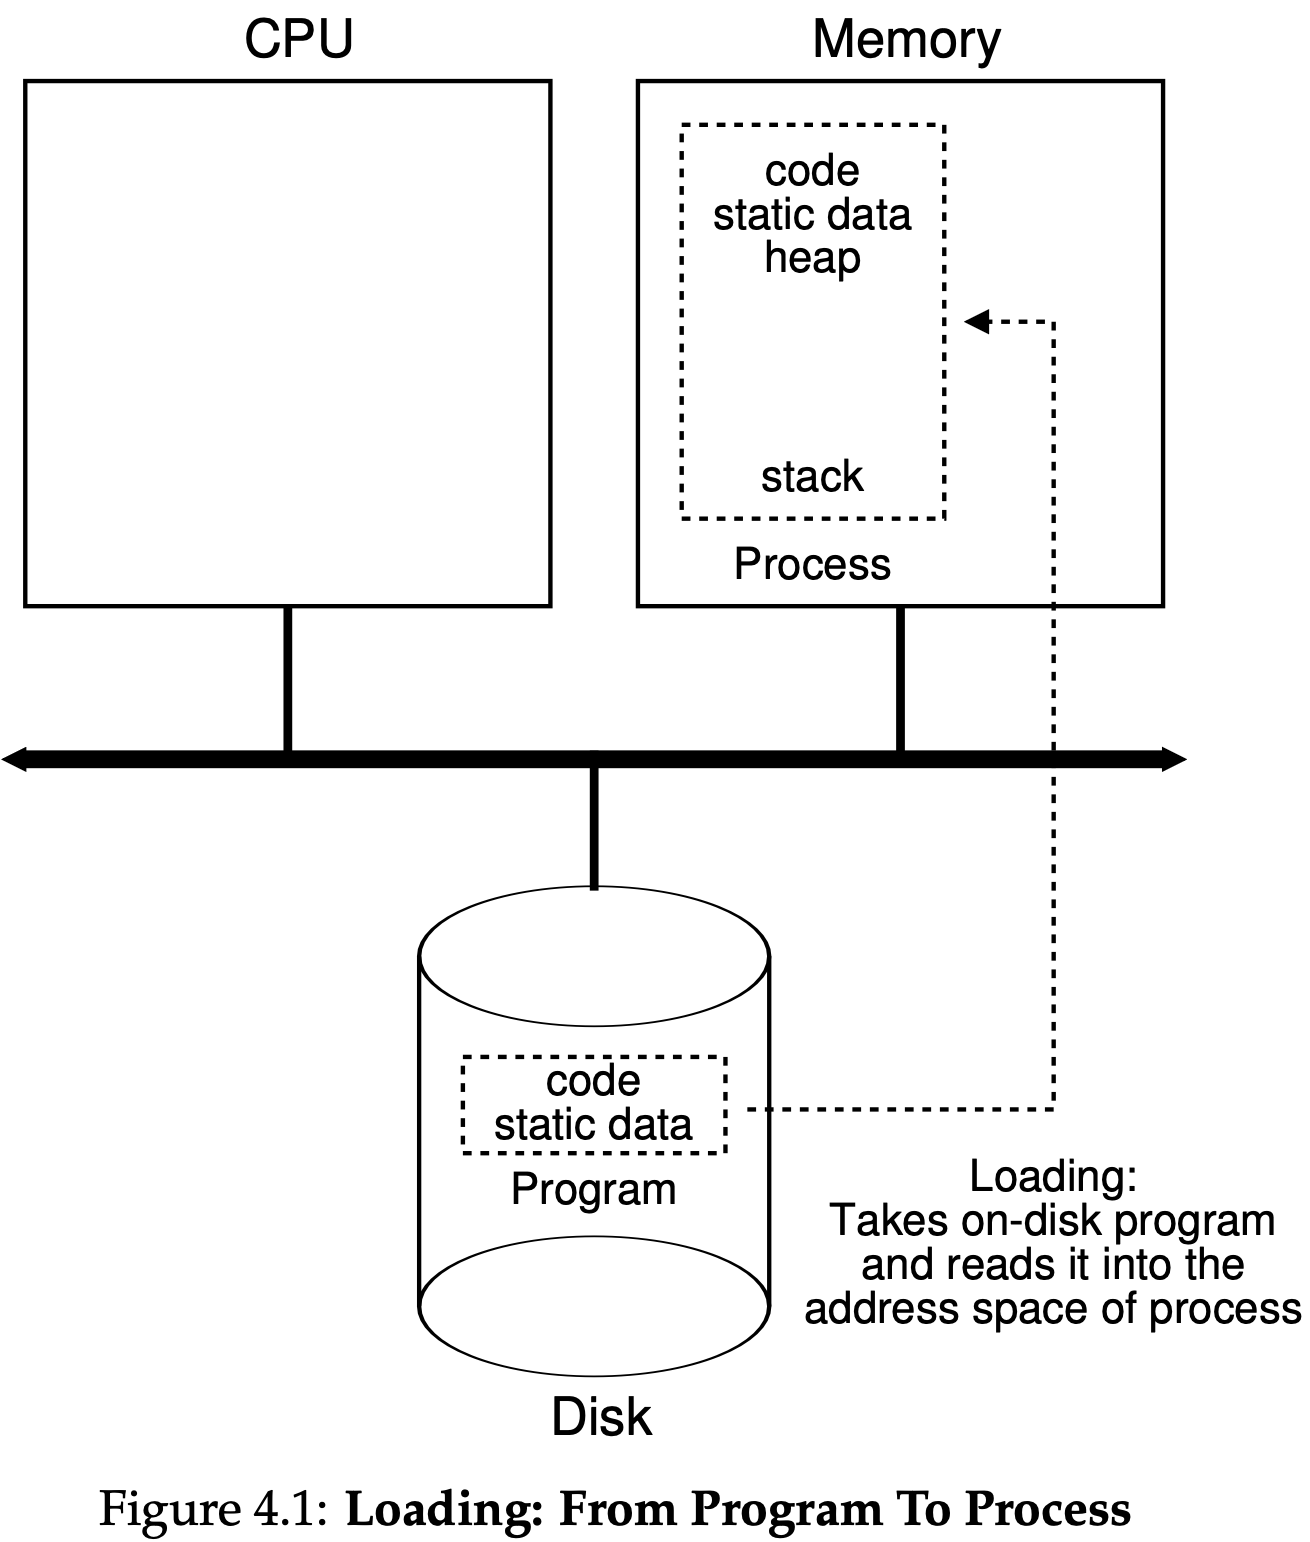
\includegraphics[width=1.1\linewidth]{figs/chapter-4/figure-4.1.png}
    \caption*{Source: chapter page 4.}
    \label{fig:figure-4.1}
\end{figure}
\end{columns}

\end{frame}

% ---------------------------------------------------------
\begin{frame}{Process Creation}

Before starting execution, the OS performs several steps:

\begin{enumerate}
    \item Load code and static data into memory.
    \item Allocate the run-time \textbf{stack}.
    \item Initialize arguments such as \texttt{argc} and \texttt{argv}.
    \item Allocate initial space for the \textbf{heap}.
    \item Initialize I/O resources.
    \item Transfer control to the program entry point.
\end{enumerate}

\vspace{0.2cm}

\begin{block}{UNIX Processes}
A process normally starts with three open file descriptors:
standard input, standard output, and standard error.
\end{block}

\end{frame}

% ---------------------------------------------------------
\begin{frame}{Loading: Eager vs. Lazy}

\begin{itemize}
    \item Early or simple operating systems may load the entire program
          before execution.
\end{itemize}

\begin{block}{Eager Loading}
Code and data are loaded into memory all at once before execution.
\end{block}

\begin{block}{Lazy Loading}
Modern systems can load pieces of code and data only when they
are needed during execution.
\end{block}

\vspace{0.2cm}

Lazy loading is related to memory virtualization mechanisms such as
paging and swapping.

\end{frame}

% ---------------------------------------------------------
\begin{frame}{Process States}

\begin{columns}

\column{0.53\textwidth}

A simplified process model contains three states:

\begin{itemize}
    \item \textbf{Running}: executing instructions on a CPU.
    \item \textbf{Ready}: able to run, but not currently selected.
    \item \textbf{Blocked}: waiting for an event, such as I/O completion.
\end{itemize}

\column{0.42\textwidth}
\begin{figure}
    \centering
    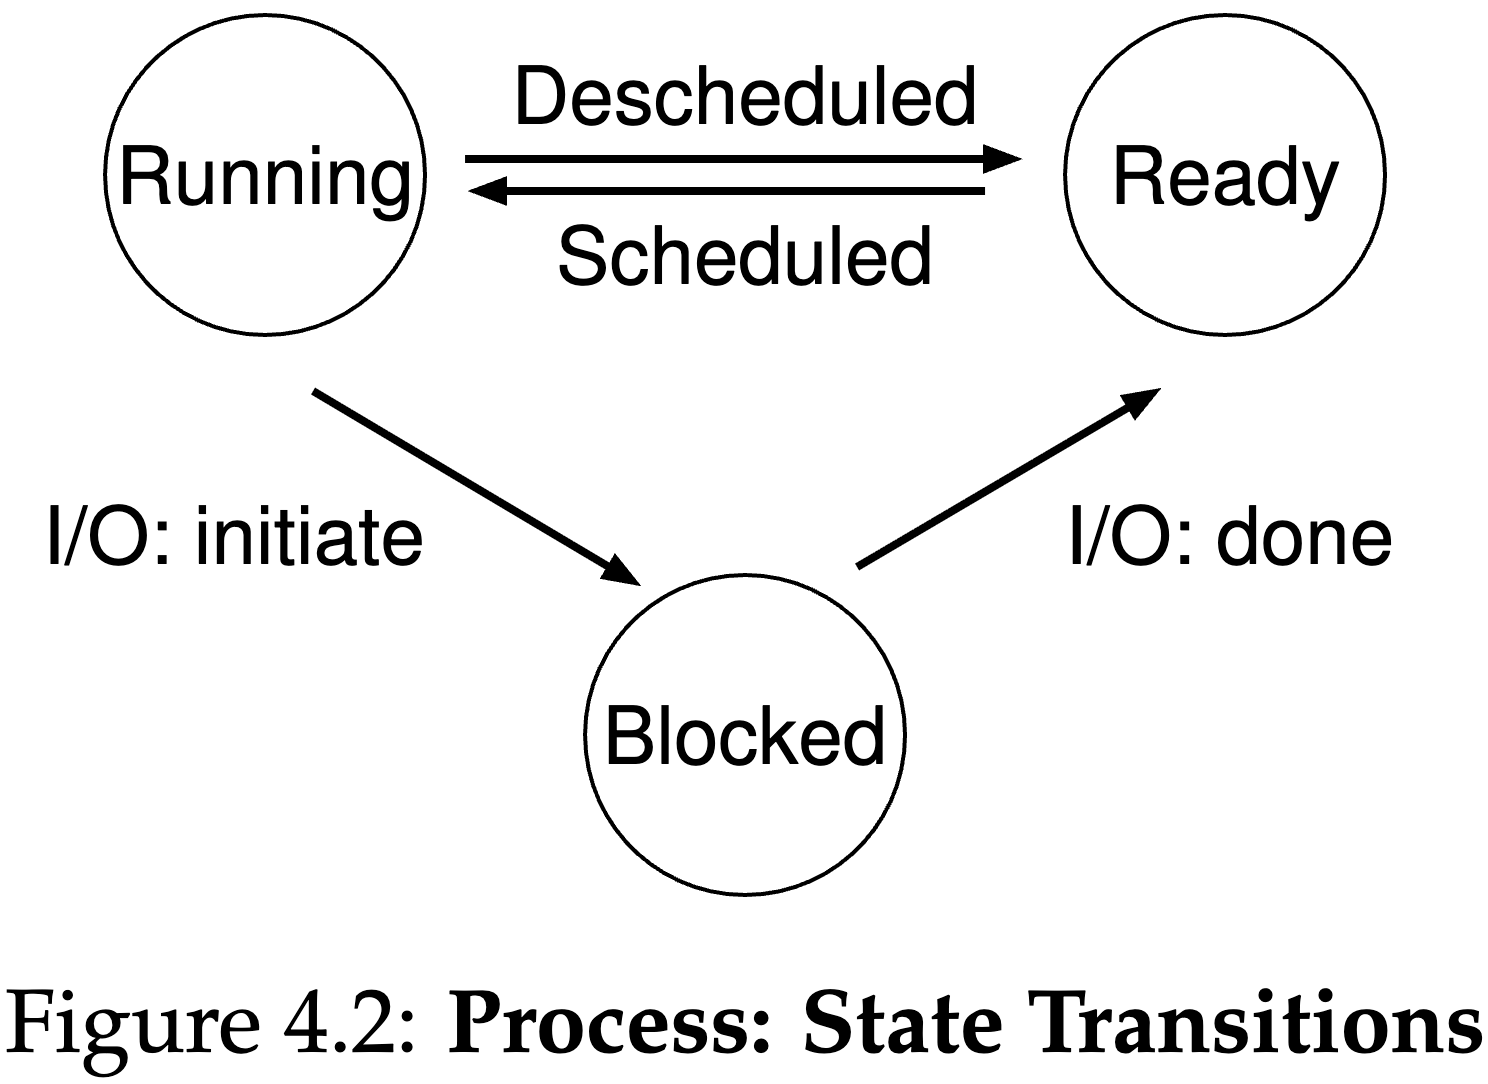
\includegraphics[width=1.1\linewidth]{figs/chapter-4/figure-4.2.png}
    \caption*{Source: chapter page 6}
    \label{fig:figure-4.2}
\end{figure}
\end{columns}

\end{frame}

% ---------------------------------------------------------
\begin{frame}{Process State Transitions}

\begin{itemize}
    \item \textbf{Ready $\rightarrow$ Running}
    \begin{itemize}
        \item the process is \textbf{scheduled}.
    \end{itemize}

    \item \textbf{Running $\rightarrow$ Ready}
    \begin{itemize}
        \item the process is \textbf{descheduled}.
    \end{itemize}

    \item \textbf{Running $\rightarrow$ Blocked}
    \begin{itemize}
        \item the process initiates an operation such as I/O.
    \end{itemize}

    \item \textbf{Blocked $\rightarrow$ Ready}
    \begin{itemize}
        \item the event or I/O operation completes.
    \end{itemize}
\end{itemize}

\end{frame}

% ---------------------------------------------------------
\begin{frame}{Example: CPU-Only Processes}

\begin{columns}

\column{0.48\textwidth}

\begin{itemize}
    \item Consider two processes that only use the CPU.
    \item One process runs while the other remains ready.
    \item When the first process finishes, the second can run.
\end{itemize}

\column{0.47\textwidth}
\begin{figure}
    \centering
    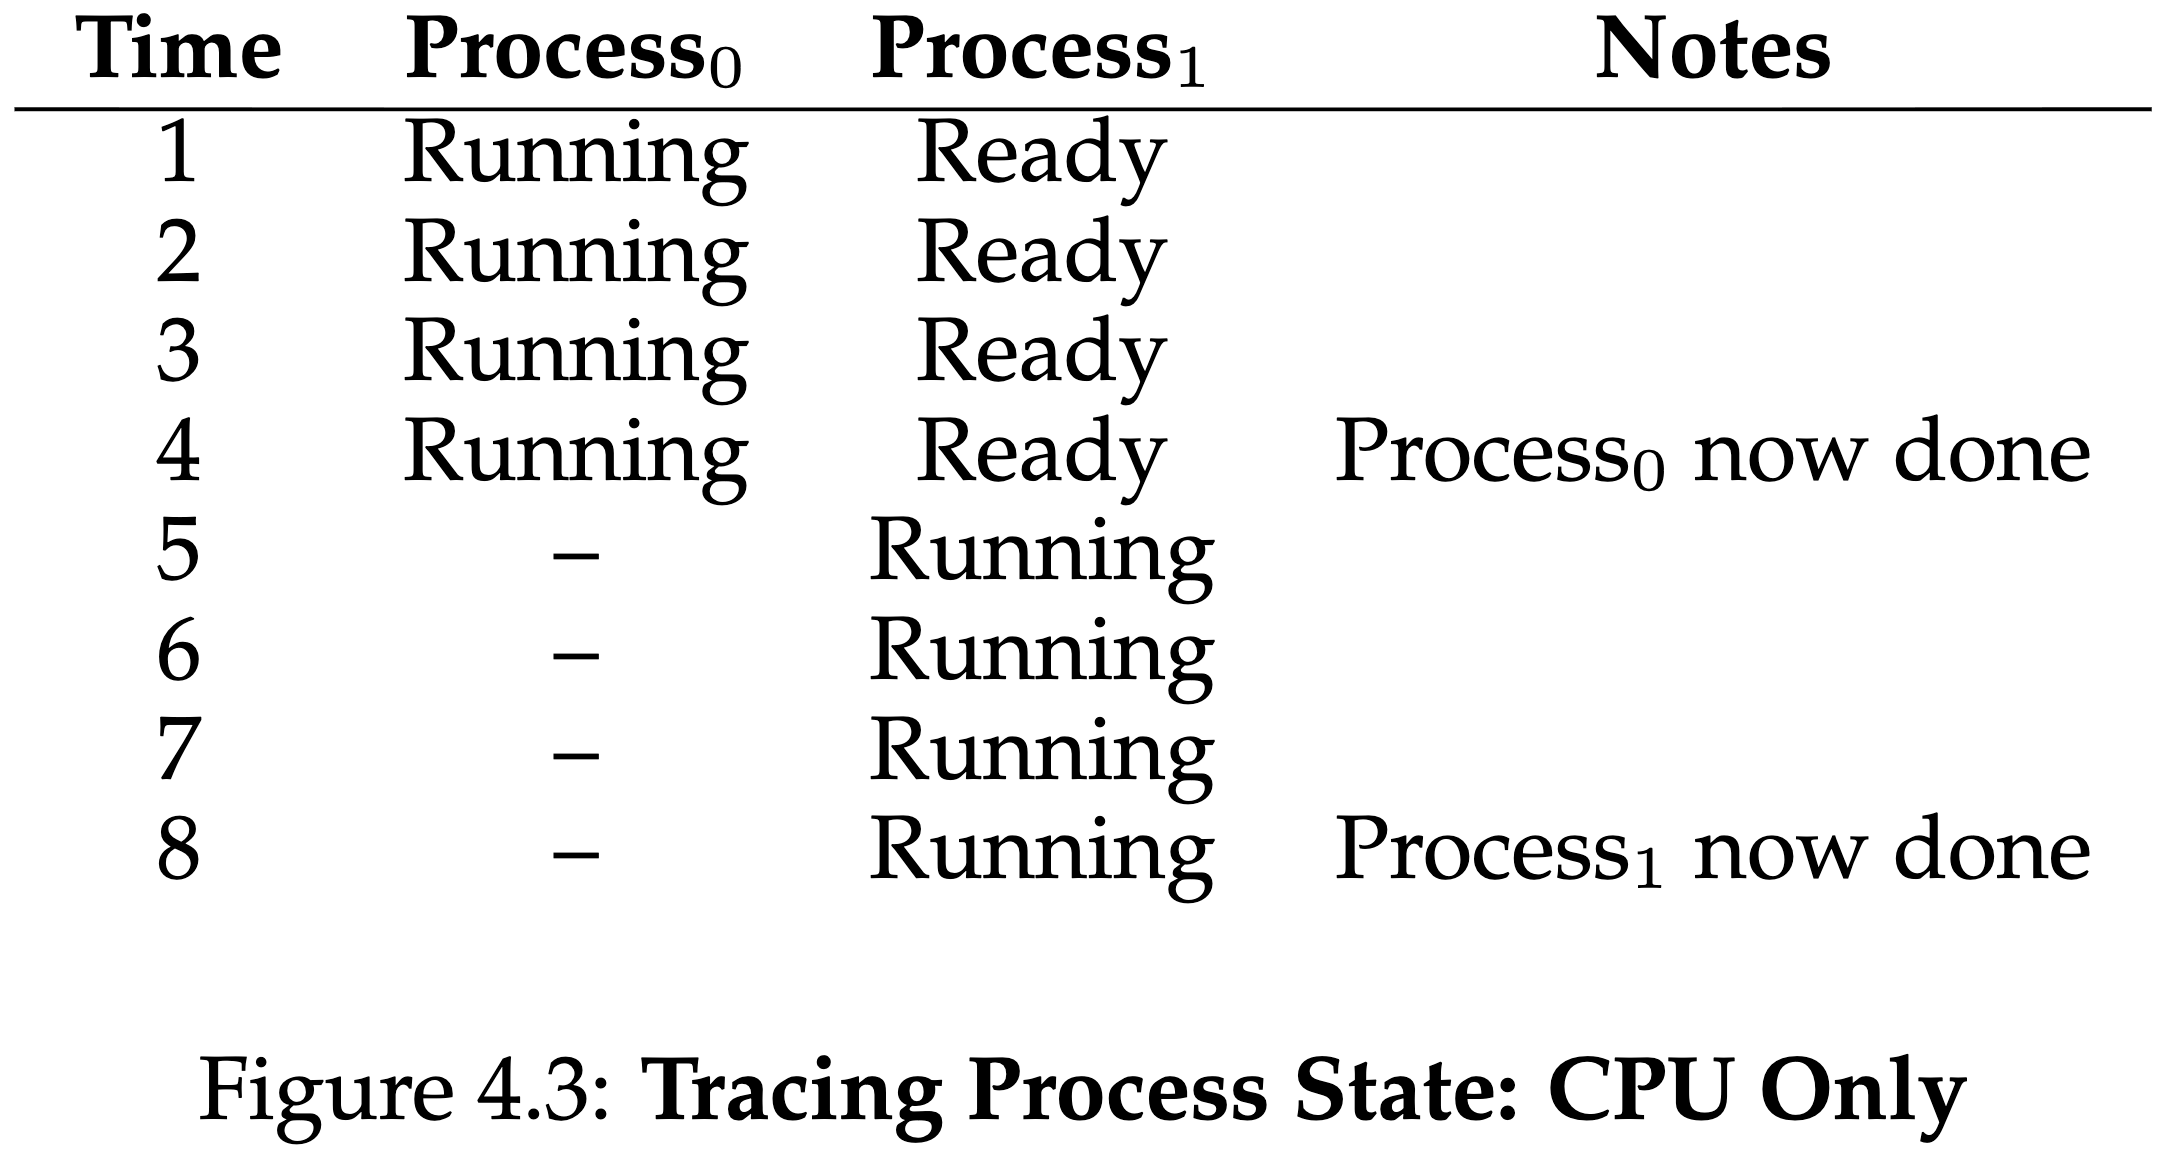
\includegraphics[width=1.1\linewidth]{figs/chapter-4/figure-4.3.png}
    \caption*{Source: chapter page 6.}
    \label{fig:figure-4.3}
\end{figure}
\end{columns}

\end{frame}

% ---------------------------------------------------------
\begin{frame}{Example: CPU and I/O}

\begin{columns}

\column{0.50\textwidth}

\begin{itemize}
    \item Process0 starts running.
    \item Process0 initiates I/O and becomes blocked.
    \item Process1 uses the CPU while Process0 waits.
    \item When I/O completes, Process0 becomes ready again.
    \item This improves CPU utilization.
\end{itemize}

\column{0.45\textwidth}
\begin{figure}
    \centering
    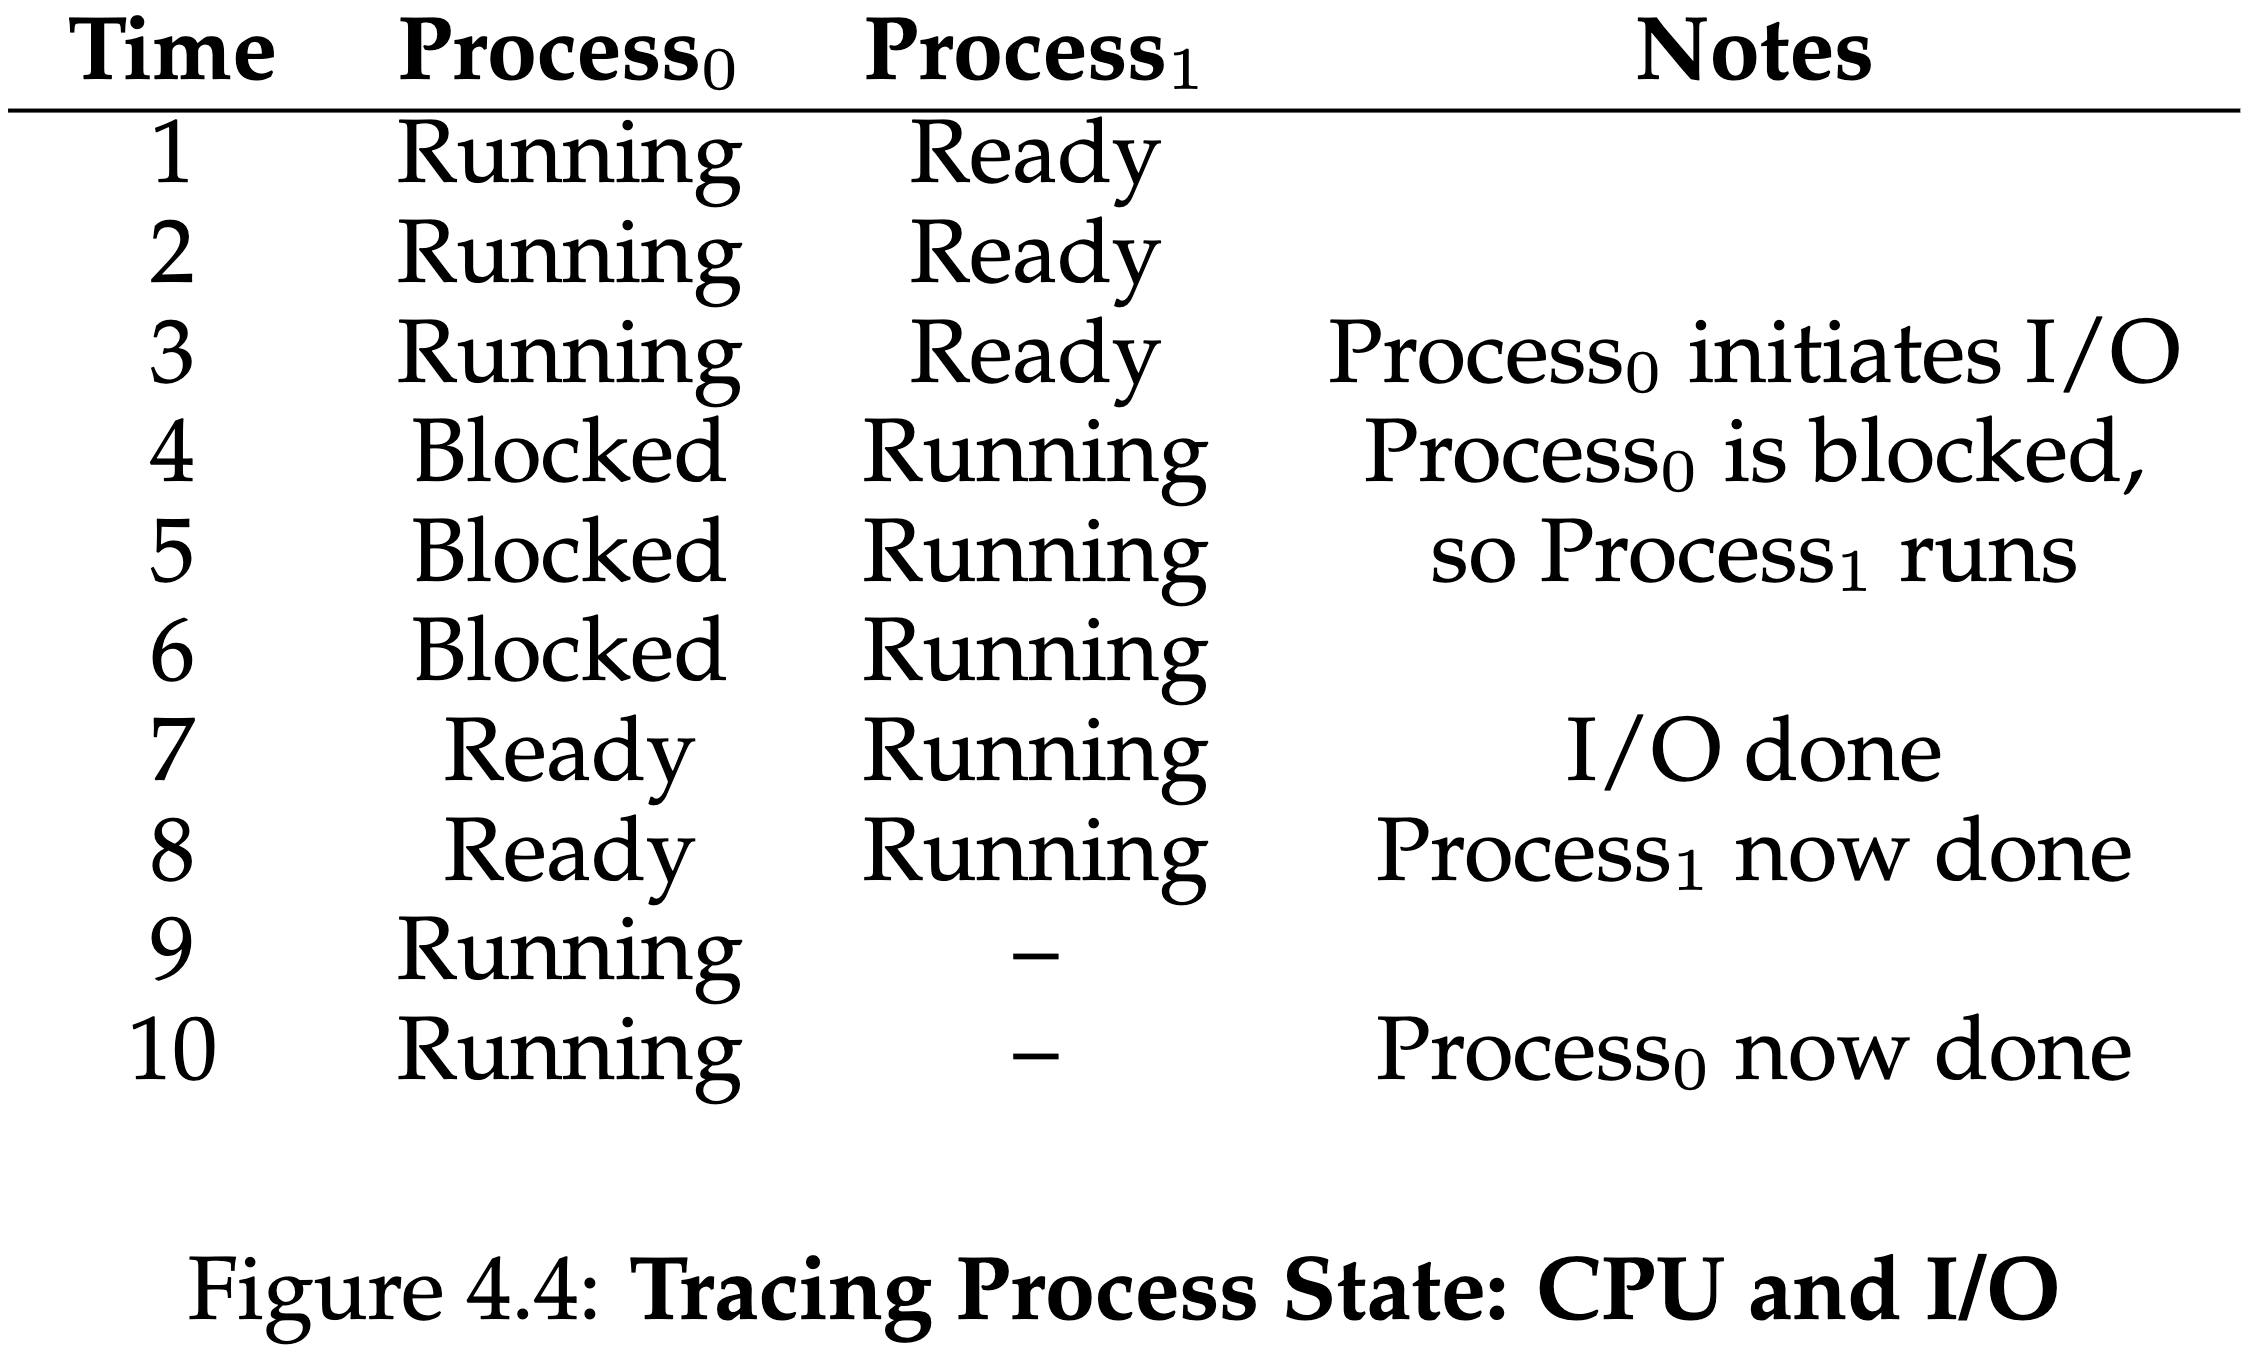
\includegraphics[width=1.1\linewidth]{figs/chapter-4/figure-4.4.png}
    \caption*{Source: chapter page 7.}
    \label{fig:figure-4.4}
\end{figure}
\end{columns}

\end{frame}

% ---------------------------------------------------------
\begin{frame}{Scheduling Decisions}

Even a simple CPU/I/O example requires OS decisions.

\begin{itemize}
    \item Which ready process should run?
    \item Should the OS switch processes when one becomes blocked?
    \item Should a process run immediately after its I/O completes?
    \item Should the currently running process continue?
\end{itemize}

\vspace{0.3cm}

\begin{block}{Scheduler}
The OS component responsible for deciding which process should
use the CPU.
\end{block}

\end{frame}

% ---------------------------------------------------------
\begin{frame}{Process Data Structures}

\begin{columns}

\column{0.48\textwidth}

The OS must keep information about every process.

\begin{itemize}
    \item process state;
    \item process identifier (PID);
    \item memory information;
    \item register context;
    \item open files;
    \item parent process;
    \item current directory.
\end{itemize}

\column{0.47\textwidth}
\begin{figure}
    \centering
    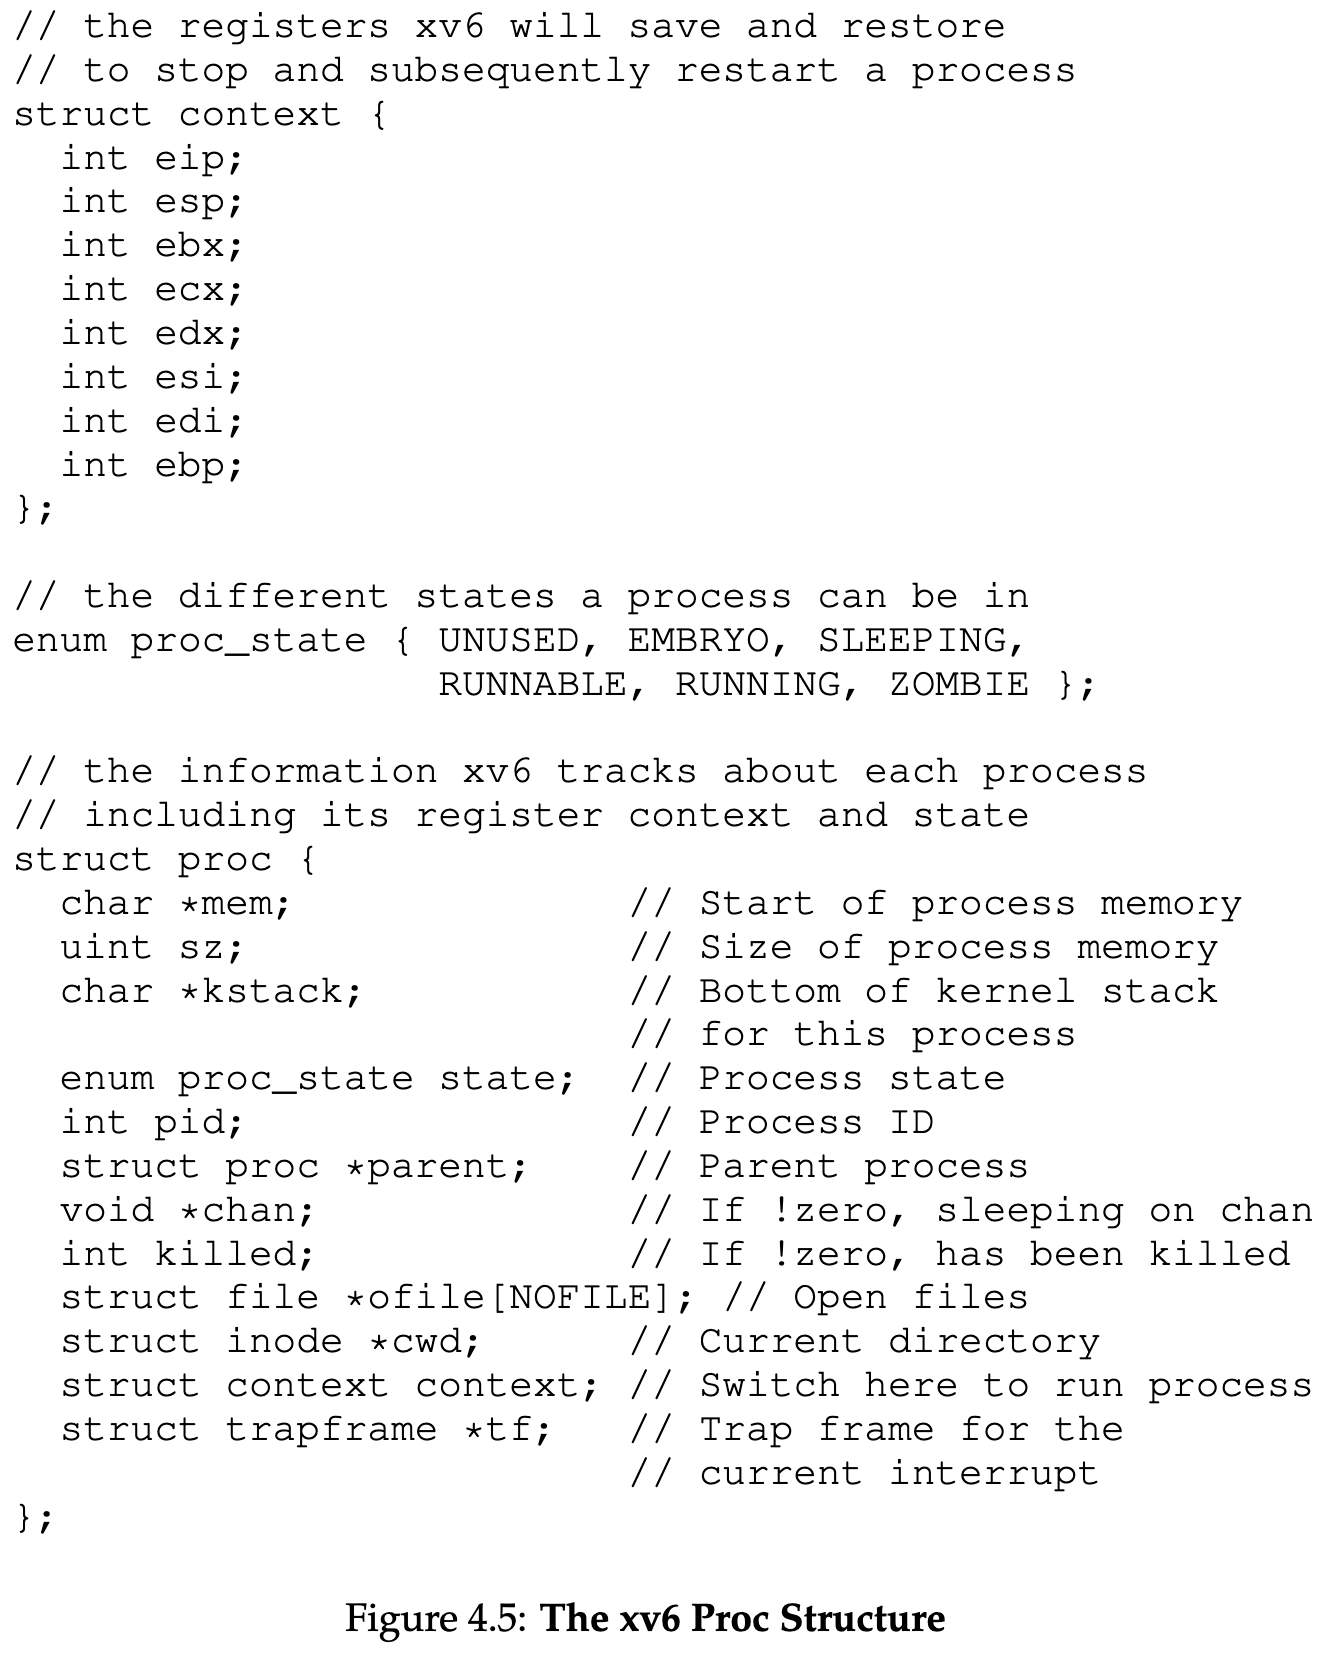
\includegraphics[width=1.1\linewidth]{figs/chapter-4/figure-4.5.png}
    \caption*{Source: chapter page 8.}
    \label{fig:figure-4.5}
\end{figure}
\end{columns}

\end{frame}

% ---------------------------------------------------------
\begin{frame}{Process List and PCB}

\begin{itemize}
    \item The OS maintains a \textbf{process list} or \textbf{task list}.
    \item It tracks:
    \begin{itemize}
        \item ready processes;
        \item running processes;
        \item blocked processes.
    \end{itemize}
    \item Information about an individual process is often stored in a
          \textbf{Process Control Block (PCB)}.
    \item The saved register context allows the OS to stop and later
          resume a process.
\end{itemize}

\begin{block}{Context Switch}
The OS saves the state of one process and restores the state
of another process.
\end{block}

\end{frame}

% ---------------------------------------------------------
\begin{frame}{Additional Process States}

Real operating systems may use more states than the simplified model.

\begin{itemize}
    \item A process may have an initial state while it is being created.
    \item A process may remain temporarily after it finishes execution.
\end{itemize}

\begin{block}{Zombie State}
In UNIX-based systems, an exited process can remain in a zombie
state until its parent obtains its return status, typically using
\texttt{wait()}.
\end{block}

\end{frame}

% ---------------------------------------------------------
\begin{frame}{Chapter Summary}

\begin{itemize}
    \item A \textbf{process} is the OS abstraction of a running program.
    \item CPU virtualization allows many processes to share a small
          number of physical CPUs.
    \item A process is characterized by:
    \begin{itemize}
        \item its address space;
        \item CPU registers;
        \item I/O state.
    \end{itemize}
    \item Processes transition among states such as
          \textbf{running}, \textbf{ready}, and \textbf{blocked}.
    \item The OS tracks processes through structures such as the
          \textbf{process list} and \textbf{PCB}.
    \item Mechanisms and policies together enable CPU virtualization.
\end{itemize}

\end{frame}